% Binary Tree Heap Example
%
% File:         binary-tree-heap.tex
% Author:       Bob Walton (walton@acm.org)
% Date:      	Mon Mar 18 20:40:50 EDT 2013
  
\documentclass{minimal}
\usepackage[paperheight=1.4in,paperwidth=2.1in,
            height=1.4in,hoffset=0.05in,
	    voffset=0.05in,left=0in,width=2.1in]{geometry}
\usepackage{color}
\usepackage[usenames]{xcolor}
\usepackage{tikz}
\usepackage{scalefnt}
\usetikzlibrary{arrows}
\begin{document}
\raggedright
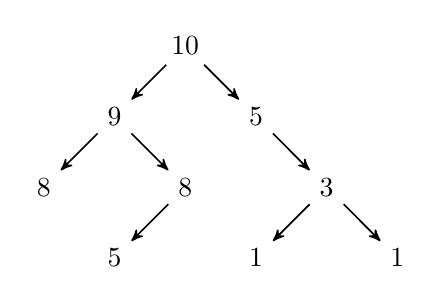
\begin{tikzpicture}[->,>=stealth',auto,
                    node distance=0.5in,semithick]
\tikzstyle{every node}=[]
\node[] (ROOT) {10};
\node (L) [below left of=ROOT] {9};
\node (LL) [below left of=L] {8};
\node (LR) [below right of=L] {8};
\node (LRL) [below left of=LR] {5};
\node (R) [below right of=ROOT] {5};
\node (RR) [below right of=R] {3};
\node (RRL) [below left of=RR] {1};
\node (RRR) [below right of=RR] {1};

\path (ROOT) edge (L) edge (R)
      (L) edge (LL) edge (LR)
      (LR) edge (LRL)
      (R) edge (RR)
      (RR) edge (RRL) edge (RRR);
\end{tikzpicture}
\end{document}

